\chapter{Spatial linear filtering}
\lecture{5}{8/11}

\begin{definition}[Mask]
    A \textbf{mask} (or \textbf{kernel}) is a small matrix that is used in many image processing techniques via \textbf{convolution} between the image and the mask.
\end{definition}

\begin{definition}[Convolution]
    \textbf{Convolution} is the process of adding each pixel to its local neighbours weighted by a mask. 
    This is a type of mathematical convolution, which will not be touched on here.
    More formally, the general expression for a convolution is
    \[ g(x, y) = \omega * f(x, y) = \sum_{i = -a}^a \sum_{j = -b}^{b} \omega(i, j) f(x + i, y + j), \]
    where $g$ is our filtered image, $\omega$ is our mask, and $f$ is our original image. Note that $\omega(i, j) \in M_{2a + 1 \times 2b + 1}(\R)$ but considered by $-a \leq i \leq a$ and $-b \leq j \leq b$.
\end{definition}

\begin{remark}
    Our processed image will have smaller dimensions due to $f(x + i, y + j)$ not being defined for $i = -1, x = 0$ (and other points on the boundary). We will look at ways to deal with this later.
\end{remark}

\begin{example}
    Consider the image represented by the following matrix
    \[
        A =
        \begin{pmatrix}
            1 & 1 & 0 & 0 \\
            1 & 1 & 0 & 0 \\
            1 & 1 & 0 & 0 \\
            1 & 1 & 0 & 0 \\
        \end{pmatrix}
    \]
    and consider the mask
    \[
        \omega =
        \begin{pmatrix}
            0 & 1  & 1 \\
            1 & -4 & 1 \\
            0 & 1  & 1 \\
        \end{pmatrix}
        .
    \]
    Find the matrix of the filtered image produced by the convolution of $A$ and $\omega$.
\end{example}

\begin{solution}
    \[
        \begin{pmatrix}
            -1 & 1 \\
            -1 & 1 \\
        \end{pmatrix}
        .
    \]
\end{solution}

\begin{example}
    Let
    \[
        A =
        \begin{pmatrix}
            0 & 0 & 0 & 0 & 0 & 0 & 0 \\
            0 & 0 & 0 & 0 & 0 & 0 & 0 \\
            0 & 0 & 1 & 1 & 0 & 0 & 0 \\
            0 & 0 & 1 & 1 & 0 & 0 & 0 \\
            0 & 0 & 0 & 0 & 0 & 0 & 0 \\
            0 & 0 & 0 & 0 & 0 & 0 & 0 \\
            0 & 0 & 0 & 0 & 0 & 0 & 0 \\
        \end{pmatrix}
        ,\qquad M =
        \begin{pmatrix}
            \sfrac19 & \sfrac19 & \sfrac19 \\
            \sfrac19 & \sfrac19 & \sfrac19 \\
            \sfrac19 & \sfrac19 & \sfrac19 \\
        \end{pmatrix}
        .
    \]
    Find the convolution of $A$ and $M$.
\end{example}

\begin{solution}
    \[
        \begin{pmatrix}
            \sfrac19 & \sfrac29 & \sfrac29 & \sfrac19 & 0 \\
            \sfrac29 & \sfrac49 & \sfrac49 & \sfrac29 & 0 \\
            \sfrac29 & \sfrac49 & \sfrac49 & \sfrac29 & 0 \\
            \sfrac19 & \sfrac29 & \sfrac29 & \sfrac19 & 0 \\
            \sfrac19 & \sfrac29 & \sfrac29 & \sfrac19 & 0 \\
        \end{pmatrix}
        .
    \]
    Note that this example is replacing each pixel with the mean of its neighbours; hence, $M$ represents a mean filter of size $3 \times 3$.
\end{solution}

\begin{definition}[Gaussian mask]
    Each value $p$ in a \textbf{Gaussian mask} is given by the Gaussian function $g$ of the distance between the element $p$ and the centre of the mask.
\end{definition}

\begin{remark}
    Recall that the Gaussian function (with $\mu = 0$) is given by
    \[ g(x) = \frac{1}{\sigma\sqrt{2\pi}} e^{-\sfrac{x^2}{2\sigma^2}}. \]
\end{remark}

\begin{example}[Gaussian mask, $n = 3$]
    Consider the following mask (where $g$ is the Gaussian function).
    \[
        \begin{pmatrix}
            g_\sigma(\sqrt 2) & g_\sigma(1) & g_\sigma(\sqrt 2) \\
            g_\sigma(1) & g_\sigma(0) & g_\sigma(1) \\
            g_\sigma(\sqrt 2) & g_\sigma(1) & g_\sigma(\sqrt 2) \\
        \end{pmatrix}
        .
    \]
    If we let $\sigma = 0.5$ we get
    \[
        \begin{pmatrix}
            0.011 & 0.083 & 0.011 \\
            0.083 & 0.619 & 0.083 \\
            0.011 & 0.083 & 0.011 \\
        \end{pmatrix}
        .
    \]
    This is a Gaussian mask.
\end{example}

\begin{remark}
    It is quite clear to see that a Gaussian mask puts much more weight towards values near the centre and less weight on the values further out.
\end{remark}

\begin{figure}
    \centering
    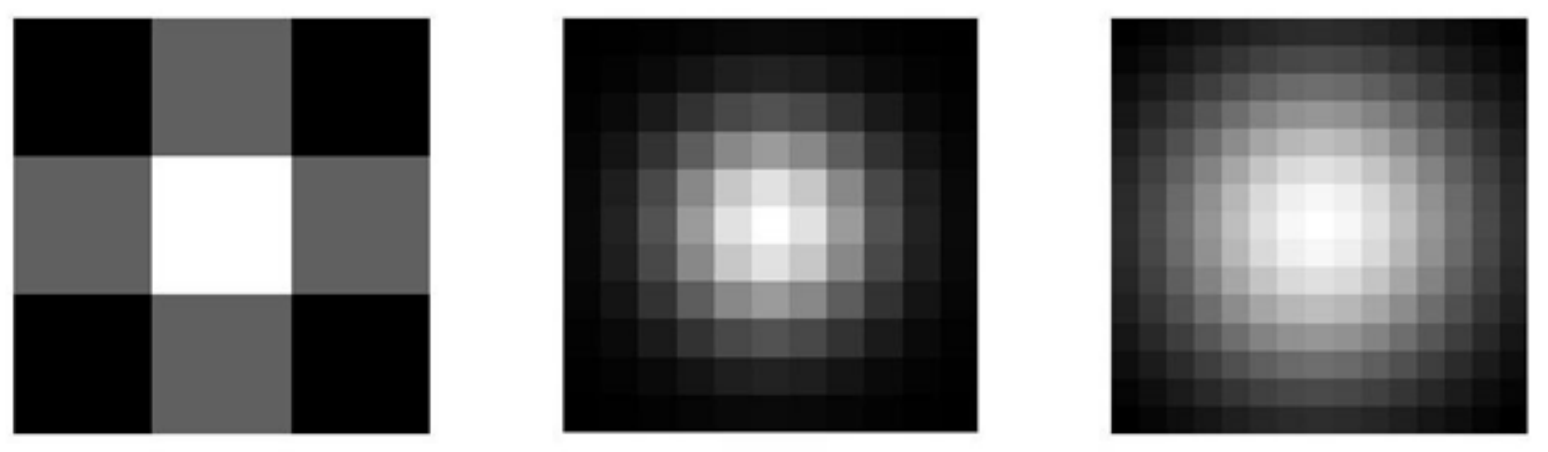
\includegraphics[width = 0.8\textwidth]{images/gaussian-mask.png}
    \caption{Grayscale visualation of Gaussian masks of various sizes.}
    \label{fig:gaussian-mask}
\end{figure}

We can also define a Gaussian filter without using a mask, if instead we want to use a general neighbours. We define
\[
    O_p = \frac{\Sigma_{p' \in \Omega} g(\lvert p - p' \rvert) I_p}{\Sigma_{p' \in \Omega} g(\lvert p - p' \rvert)}.
\]
The denominator here acts just to normalise the expression (so all the sums weight to 1).

\begin{remark}
    Gaussian filters are typically used to remove noise, but it also \emph{blurs} and \emph{smoothes} the image. That is, it removes fine details. \emph{This is a key remark.}
\end{remark}

\begin{figure}
    \centering
    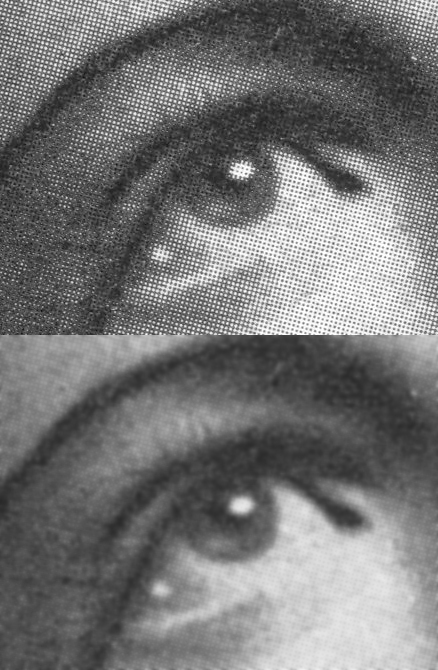
\includegraphics[width=0.4\linewidth]{images/gaussian-filter.jpg}
    \caption{Example of an image that has had a Gaussian filter (Gaussian blur) applied to it (compared to the original above).}
    \label{fig:gaussian-filter}
\end{figure}

\begin{remark}
    As we increase $\sigma$ we get a more blurred image, see one of the figures around here.
\end{remark}

\begin{figure}
    \centering
    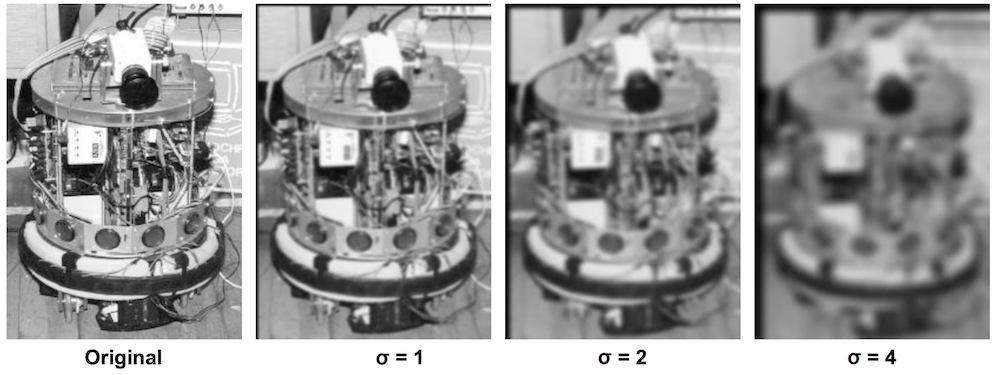
\includegraphics[width=0.8\linewidth]{images/gaussian-increase-sigma.png}
    \caption{Comparison of blurring effect as $\sigma$ increases.}
    \label{fig:gaussian-increase-sigma}
\end{figure}

There are two techniques that can be used to combat the issue of blurring that comes from Gaussian filters: \emph{non-local means} and \emph{bilateral filtering}.

\begin{definition}[Non-local means]
    \textbf{Non-local means} is an algorithm that takes means of every pixel in the image weighted by how similar the pixel is to the target pixel. 
\end{definition}

The performance of non-local means is not fantastic, depending on the size of the neighbour we take the means from (as it could just be a subset of the full image); however, there exists optimisations and it is easily made parallel (each pixel can be done in parallel).

We will now look at convolution using a \emph{Laplacian mask}... first some mathematics.

\begin{definition}[Laplacian]
    The Laplacian of a function $f(x, y)$ in cartesian coordinates is defined as
    \[ \Delta f = \frac{\partial^2f}{\partial x^2} + \frac{\partial^2f}{\partial y^2}. \]
\end{definition}

You have seen that we treat images like functions; however, the Laplacian is only defined for continuous functions and our images are discrete. So, instead of looking at the second partial derivate we just look at the differences. Consider the matrix
\[
    \begin{pmatrix}
        a & b & c
    \end{pmatrix}
    .
\]
Then we get the differences $\begin{pmatrix} b - a & c - b \end{pmatrix}$. Taing the differences of these differences (to get our second order) we get $c - b - b - a = c - 2b + a$. This is identical to the convolution of the above matrix and $\begin{pmatrix} 1 & -2 & 1 \end{pmatrix}$; hence is called the \textbf{Laplacian mask}.

So in a 2D image we just add the $x$ differences and $y$ differences to get the mask
\[
    \begin{pmatrix}
        0 & 1 & 0 \\
        1 & -4 & 0 \\
        0 & 1 & 0 \\
    \end{pmatrix}
    .
\]

Now, if an image changes consistently (such as a gradient) then the convolution with a Laplacian mask will always be full of zeros. So we only see (significant) non-zero values when there is inconsistent change, that is, near \emph{edges}. This is what Laplacian filtering is good for; edge detection.

We can also subtract the Laplacian filtered image from itself to get a sharpening effect.

\begin{figure}
    \centering
    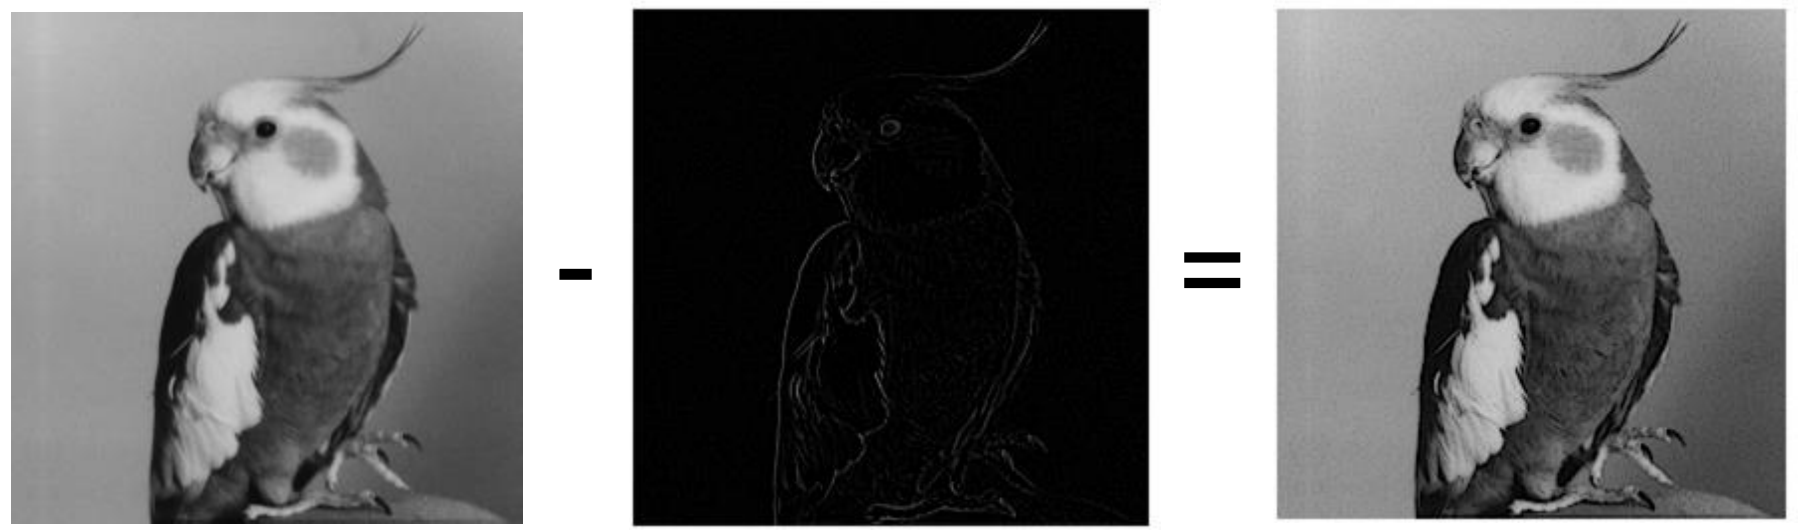
\includegraphics[width=0.8\linewidth]{images/sharpening-laplacian}
    \caption{Example of sharpening with a Laplacian filter.}
    \label{fig:sharpening-laplacian}
\end{figure}

\begin{remark}
    Laplacian filtering is sensitive to noise; however, to avoid excessive noise we can compute the Laplacian of a Gaussian blurred image.
\end{remark}

Now, one final point. What do we do at image boundaries? We have a few options...
\begin{enumerate}
    \item We can treat them as zeros. This is typically a terrible choice visually.
    \item Extrapolate from values in the image (best option).
    \item Do not perform convolution on these parts of the image (leads to images of smaller dimensions).
\end{enumerate}
